\PassOptionsToPackage{unicode}{hyperref}
\PassOptionsToPackage{hyphens}{url}
\documentclass{article}
\setcounter{secnumdepth}{3}

\usepackage{amsmath,amssymb}
\usepackage{lmodern}
\usepackage{iftex}
\usepackage[letterpaper, margin=1in, top=1in, bottom=2in]{geometry}
\usepackage{listings}
\usepackage{color}
\usepackage{titling}
\usepackage{graphicx}
\usepackage{hyperref}

\ifPDFTeX
  \usepackage[T1]{fontenc}
  \usepackage[utf8]{inputenc}
  \usepackage{textcomp} 
\else 
  \usepackage{unicode-math}
  \defaultfontfeatures{Scale=MatchLowercase}
  \defaultfontfeatures[\rmfamily]{Ligatures=TeX,Scale=1}
\fi
\IfFileExists{upquote.sty}{\usepackage{upquote}}{}
\IfFileExists{microtype.sty}{
  \usepackage[]{microtype}
  \UseMicrotypeSet[protrusion]{basicmath} 
}{}
\makeatletter
\@ifundefined{KOMAClassName}{
  \IfFileExists{parskip.sty}{
    \usepackage{parskip}
  }{
    \setlength{\parindent}{0pt}
    \setlength{\parskip}{6pt plus 2pt 2pt}}
}{
  \KOMAoptions{parskip=half}}
\makeatother
\usepackage{xcolor}
\usepackage{graphicx}

\makeatletter
\def\maxwidth{\ifdim\Gin@nat@width>\linewidth\linewidth\else\Gin@nat@width\fi}
\def\maxheight{\ifdim\Gin@nat@height>\textheight\textheight\else\Gin@nat@height\fi}
\makeatother
\setkeys{Gin}{width=\maxwidth,height=\maxheight,keepaspectratio}
\makeatletter
\def\fps@figure{htbp}
\makeatother
\setlength{\emergencystretch}{3em} 
\providecommand{\tightlist}{
  \setlength{\itemsep}{0pt}\setlength{\parskip}{0pt}}

\ifLuaTeX
  \usepackage{selnolig}  
\fi
\IfFileExists{bookmark.sty}{\usepackage{bookmark}}{\usepackage{hyperref}}
\IfFileExists{xurl.sty}{\usepackage{xurl}}{} 
\urlstyle{same}
\hypersetup{
  hidelinks,
  pdfcreator={LaTeX via pandoc}}

\title{Methodology}
\author{}
\date{}

\begin{document}

\maketitle

\hypertarget{roles}{
\section{Roles}\label{roles}}

\hypertarget{teamleadarchitect}{
\subsection{Team Lead \& Architect}\label{teamleadarchitect}}

\textbf{Team Lead:}
Fabian Romero Claros

\textbf{Architect:}
Gabriel Santiago Concha Saavedra

\begin{center}\rule{0.5\linewidth}{0.5pt}\end{center}

\hypertarget{sprint0}{
\subsection{Sprint 0}\label{sprint0}}

\textbf{Product Owner:}
Emanuel Galindo Corpa 

\textbf{Scrum Master: }
Jose Luis Terán Rocha

\hypertarget{qateam}{
\subsubsection{QA Team}\label{qateam-0}}

\begin{itemize}
\tightlist
\item
  Ronaldo Miguel Ángel Mendoza Mallcu
\item
  Sebastián Barra Zurita
\item
  Jhael Arce Chavez
\end{itemize}

\hypertarget{devteam}{
\subsubsection{Dev Team}\label{devteam-0}}

\begin{itemize}
\tightlist
\item
  Fabian Romero Claros
\item
  Gabriel Santiago Concha Saavedra
\item
  Josue Mauricio Prado Camacho
\item
  Luis Enrique Espinoza Vera
\item
  Luiggy Mamani Condori
\item
  Axel Javier Ayala Siles
\item
  Victor Leon Villca Silva
\item
  Alex Paca Meneses
\item
  Jose Luis Terán Rocha
\end{itemize}

\begin{center}\rule{0.5\linewidth}{0.5pt}\end{center}

\hypertarget{sprint1}{
\subsection{\texorpdfstring{\textbf{Sprint
1}}{Sprint 1}}\label{sprint1}}

\textbf{Product Owner: }
Alex Paca Meneses

\textbf{Scrum Master: }
Jose Luis Terán Rocha

\hypertarget{qateam-1}{
\subsubsection{\texorpdfstring{\textbf{QA Team}}{QA Team}}\label{qateam-1}}

\begin{itemize}
\tightlist
\item
  Jhael Arce Chavez - \textbf{QA Lead}
\item
  Sebastian Barra Zurita
\item
  Ronaldo Miguel Angel Mendoza Mallcu
\end{itemize}

\hypertarget{devteam-1}{
\subsubsection{\texorpdfstring{\textbf{Dev
Team}}{Dev Team}}\label{devteam-1}}

\paragraph{Front End Team}\label{front-end-team-1}

\begin{itemize}
\tightlist
\item
  Victor Leon Villca Silva ~- \textbf{Lead}
\item
  Emanuel Javier Galindo Corpa
\item
  Luis Enrique Espinoza Vera
\item
  Josue Mauricio Prado Camacho
\end{itemize}

\paragraph{Back End Team}\label{back-end-team-1}

\begin{itemize}
\tightlist
\item
  Alex Paca Meneses \textbf{- Lead}
\item
  Gabriel Santiago Concha Saavedra
\item
  Axel Javier Ayala Siles
\item
  Fabian Romero Claros
\item
  Luiggy Mamani Condori
\item
  Jose Luis Terán Rocha
\end{itemize}

\subsubsection{DevOps / Infrastructure Team}\label{devops-team-1}

\begin{itemize}
\tightlist
\item
  Gabriel Santiago Concha Saavedra
\item
  Jose Luis Terán Rocha
\end{itemize}

\begin{center}\rule{0.5\linewidth}{0.5pt}\end{center}

\hypertarget{sprint2}{
\subsection{\texorpdfstring{\textbf{Sprint
2}}{Sprint 2}}\label{sprint2}}

\textbf{Product Owner: }
Alex Paca Meneses

\textbf{Scrum Master: }
Jose Luis Terán Rocha

\hypertarget{qateam-2}{
\subsubsection{\texorpdfstring{\textbf{QA Team}}{QA Team}}\label{qateam-2}}

\begin{itemize}
\tightlist
\item
  Ronaldo Miguel Angel Mendoza Mallcu ~- \textbf{QA Lead}
\item
  Jhael Arce Chavez
\item
  Sebastian Barra Zurita
\end{itemize}

\hypertarget{devteam-2}{
\subsubsection{\texorpdfstring{\textbf{Dev
Team}}{Dev Team}}\label{devteam-2}}

\paragraph{Front End Team}\label{front-end-team-2}

\begin{itemize}
\tightlist
\item
  Emanuel Javier Galindo Corpa - \textbf{Lead}
\item
  Victor Leon Villca Silva
\item
  Luis Enrique Espinoza Vera
\item
  Josue Mauricio Prado Camacho
\end{itemize}

\paragraph{Back End Team}\label{back-end-team-2}

\begin{itemize}
\tightlist
\item
  Axel Javier Ayala Siles - \textbf{Lead}
\item
  Gabriel Santiago Concha Saavedra
\item
  Alex Paca Meneses
\item
  Fabian Romero Claros
\item
  Luiggy Mamani Condori
\item
  Jose Luis Terán Rocha
\end{itemize}

\subsubsection{DevOps / Infrastructure Team}\label{devops-team-2}

\begin{itemize}
\tightlist
\item
  Gabriel Santiago Concha Saavedra
\item
  Jose Luis Terán Rocha
\end{itemize}

\begin{center}\rule{0.5\linewidth}{0.5pt}\end{center}

\hypertarget{sprint3}{
\subsection{\texorpdfstring{\textbf{Sprint
3}}{Sprint 3}}\label{sprint3}}

\textbf{Product Owner:}
Alex Paca Meneses

\textbf{Scrum Master:}
Jose Luis Terán Rocha

\hypertarget{qateam-3}{
\subsubsection{\texorpdfstring{\textbf{QA Team}}{QA Team}}\label{qateam-3}}

\begin{itemize}
\tightlist
\item
  Josue Mauricio Prado Camacho ~- \textbf{QA Lead}
\item
  Luis Enrique Espinoza Vera
\end{itemize}

\hypertarget{devteam-3}{
\subsubsection{\texorpdfstring{\textbf{Dev
Team}}{Dev Team}}\label{devteam-3}}

\paragraph{Games Team}\label{games-team-3}

\begin{itemize}
\tightlist
\item
  Fabian Romero Claros ~-
  \textbf{Lead}
\item
  Ronaldo Miguel Angel Mendoza Mallcu
\item
  Jhael Arce Chavez
\item
  Victor Leon Villca Silva
\item
  Emanuel Galindo Corpa
\item
  Sebastian Barra Zurita
\end{itemize}

\paragraph{Console Team}\label{console-team-3}

\begin{itemize}
\tightlist
\item
  Luiggy Mamani Condori ~- \textbf{Lead}
\item
  Gabriel Santiago Concha Saavedra
\item
  Alex Paca Meneses
\item
  Axel Javier Ayala Siles
\item
  Jose Luis Terán Rocha
\end{itemize}

\subsubsection{DevOps / Infrastructure Team}\label{devops-team-3}

\begin{itemize}
\tightlist
\item
  Gabriel Santiago Concha Saavedra
\item
  Jose Luis Terán Rocha
\end{itemize}

\begin{center}\rule{0.5\linewidth}{0.5pt}\end{center}

\hypertarget{sprint4}{
\subsection{\texorpdfstring{\textbf{Sprint
4}}{Sprint 4}}\label{sprint4}}

\textbf{Product Owner: }
Alex Paca Meneses

\textbf{Scrum Master: }
Ronaldo Miguel Angel Mendoza Mallcu

\hypertarget{devteam-4}{
\subsubsection{\texorpdfstring{\textbf{Dev
Team}}{Dev Team}}\label{devteam-4}}

\paragraph{Games Team}\label{games-team-4}

\begin{itemize}
\tightlist
\item
  Fabian Romero Claros - \textbf{Lead}
\item
  Ronaldo Miguel Angel Mendoza Mallcu
\item
  Jhael Arce Chavez
\item
  Victor Leon Villca Silva
\item
  Emanuel Galindo Corpa
\item
  Sebastian Barra Zurita
\end{itemize}

\paragraph{Console Team}\label{console-team-4}

\begin{itemize}
\tightlist
\item
  Luiggy Mamani Condori - \textbf{Lead}
\item
  Gabriel Santiago Concha Saavedra
\item
  Alex Paca Meneses
\item
  Jose Luis Terán Rocha
\item
  Josue Mauricio Prado Camacho
\item
  Luis Enrique Espinoza Vera
\item
  Axel Javier Ayala Siles
\end{itemize}

\subsubsection{DevOps / Infrastructure Team}\label{devops-team-4}

\begin{itemize}
\tightlist
\item
  Gabriel Santiago Concha Saavedra
\item
  Jose Luis Terán Rocha
\end{itemize}

\newpage

\hypertarget{ceremonies}{
\section{CEREMONIES}\label{ceremonies}}

\hypertarget{scrumofscrums}{
\subsection{Scrum of Scrums}\label{scrumofscrums}}

We will implement a Scrum of Scrums approach to facilitate coordination
among multiple teams. This will involve regular meetings among the team
leads to discuss progress, dependencies, and impediments that affect the
larger project.\\
We will work using the agile framework, so our ceremonies will be the
following:~

\hypertarget{dailyleadstandup}{
\subsection{Daily Lead Stand Up}\label{dailyleadstandup}}

To ensure coordination among team leads, we will have daily stand-up
meetings specifically for the leads of each sub-team, the team lead, the
PO and the architect.. These meetings will focus on high-level updates,
strategic decisions, and any cross-team dependencies or issues. The
meeting will be on Tuesdays and Thursdays after finishing the daily
stand ups of all the teams.

\hypertarget{sprintplanning}{
\subsection{Sprint Planning:}\label{sprintplanning}}

Every Monday will be our meetings where Dev and QA Team will follow the
next points:

\begin{itemize}
\tightlist
\item
  Use of \textbf{Poker Planning} to estimate the points of each US.

  \begin{itemize}
  \tightlist
  \item
    The story points will be defined by the complexity of development
    and QA team.
  \end{itemize}
\item
  While we are defining our \textbf{Sprint Goals} and prioritize of new
  US to work

  \begin{itemize}
  \tightlist
  \item
    During the meeting, we will clarify any ambiguities or doubts about
    the US, which can conduce to a refinement of the US that is
    considered as \textbf{Backlog Refinement} or \textbf{Backlog
    Grooming.}
  \end{itemize}
\end{itemize}

\hypertarget{sprintduration}{
\subsection{\texorpdfstring{\textbf{Sprint
Duration:}}{Sprint Duration:}}\label{sprintduration}}

\begin{itemize}
\tightlist
\item
  As a team, we define our sprint of 1 weeks.
\end{itemize}

\hypertarget{dailystandup}{
\subsection{Daily Stand Up:}\label{dailystandup}}

Daily stand-up meetings will be held by each sub-team to communicate
progress and discuss any roadblocks. The schedule for these daily
stand-ups will be set and agreed upon by each sub-team. The Scrum Master
must attend all daily stand-up meetings.

\hypertarget{demodelivery}{
\subsection{Demo - Delivery:}\label{demodelivery}}

Every Friday will be our demo about the US worked during the Sprint.

\begin{itemize}
\tightlist
\item
  Having the demo of the product and the report and metrics of QA Team
  during the Sprint.

  \begin{itemize}
  \tightlist
  \item
    In the final demo will present the entire product developed with
    some metrics about US and also, the whole metrics by QA Team.
  \end{itemize}
\end{itemize}

\hypertarget{sprintreview}{
\subsection{Sprint Review:}\label{sprintreview}}

Every Friday will take into account the following points:

\begin{itemize}
\tightlist
\item
  Review of the work that has been completed during the sprint.

  \begin{itemize}
  \tightlist
  \item
    What items have been completed?
  \item
    Do we some US for Carry Over?
  \end{itemize}
\item
  \textbf{Review of the Product Backlog:}

  \begin{itemize}
  \tightlist
  \item
    Current state of the product backlog, what items remains.
  \item
    Changes are made based on the feedback received by Dev and QA Team
    and any changes according PO needs.
  \end{itemize}
\item
  The team and PO will collaborate on what to work on next, helping to
  prioritize the next sprint's backlog.
\item
  We will review what US did not go well in the Sprint and how we will
  fix it.
\end{itemize}

\hypertarget{sprintretrospective}{
\subsection{Sprint Retrospective:}\label{sprintretrospective}}

Every Friday when finishing the Sprint, where we are gonna talk about
what went right, what went wrong and what can be improved for our next
iteration. Having feedback from the sprint review.

\begin{itemize}
\tightlist
\item
  While the meeting is happening, we will work on our \textbf{Action
  Items}.

  \begin{itemize}
  \tightlist
  \item
    Identifing things we should start doing, stop doing, and continue
    doing in future Sprints, as well as specific action items to
    implement these changes.
  \end{itemize}
\end{itemize}

\newpage

\hypertarget{artifacts}{
\section{ARTIFACTS}\label{artifacts}}

\hypertarget{productbacklog}{
\subsection{\texorpdfstring{\textbf{Product
Backlog}}{Product Backlog}}\label{productbacklog}}

We maintain a prioritized list of all the features, enhancements, bug
fixes, and other work needed to complete the project.
It\textquotesingle s our single source of truth for what needs to be
done.

\hypertarget{sprintbacklog}{
\subsection{\texorpdfstring{\textbf{Sprint
Backlog}}{Sprint Backlog}}\label{sprintbacklog}}

We select a subset of the Product Backlog items for a specific Sprint,
along with a plan for how to deliver them. It\textquotesingle s created
during the Sprint Planning meeting by the Development Team and serves as
a guide for our work during the Sprint.

\hypertarget{burndownchart}{
\subsection{\texorpdfstring{\textbf{Burn-Down
Chart}}{Burn-Down Chart}}\label{burndownchart}}

We use a representation of the amount of work remaining in the Sprint.
It shows our progress towards completing the Sprint\textquotesingle s
goal and helps us track whether we\textquotesingle re on track to finish
all planned work by the end of the Sprint.

\hypertarget{impedimentlog}{
\subsection{\texorpdfstring{\textbf{Impediment
Log}}{Impediment Log}}\label{impedimentlog}}

We keep a record of the impediments or problems of each team member per
day It\textquotesingle s used during our Daily Standup meeting to
~identify any issues that need to be addressed.

\hypertarget{startstopcontinueactionitems}{
\subsection{\texorpdfstring{\textbf{Start-Stop-Continue-Action
Items}}{Start-Stop-Continue-Action Items}}\label{startstopcontinueactionitems}}

We identify things we should start doing, stop doing, and continue doing
in future Sprints, as well as specific action items to implement these
changes. It helps us reflect on our process and make improvements for
future iterations.

\newpage

\hypertarget{dordod}{
\section{DOR/DOD}\label{dordod}}

\hypertarget{definitionofready}{
\subsection{\texorpdfstring{\textbf{Definition of
Ready}}{Definition of Ready}}\label{definitionofready}}

\begin{itemize}
\tightlist
\item
  The story should have a clear description that indicates what it hopes
  to achieve and why it is important.
\item
  Clear criteria should be established indicating when the user story
  will be considered complete.
\item
  The necessary resources (such as people, tools) must be available to
  complete the story effectively.
\item
  Before a story can be considered ready for development, it must have
  been prioritized and estimated.
\end{itemize}

\hypertarget{definitionofdone}{
\subsection{\texorpdfstring{\textbf{Definition of
Done}}{Definition of Done}}\label{definitionofdone}}

\begin{itemize}
\tightlist
\item
  Code reviews must be performed by at least one and max two team
  members.
\item
  All issues identified during the code review should be fixed.
\item
  Unit Tests must be completed and successfully passed before a task is
  considered ready for delivery.
\item
  All methods and classes from the library must be documented.
\item
  The documentation in the library provided should be clear, concise, and adequately
  describe the functionality of the code.
\item
  The architecture defined by the team must be followed, including
  established design patterns and conventions.
\end{itemize}

\newpage

\hypertarget{workflow-gitflow}{
\section{WORKFLOW AND GITFLOW:}\label{workflow-gitflow}}

\hypertarget{workflow}{
\subsection{Workflow:}\label{workflow}}

\hypertarget{availabilitysupporttime}{
\subsubsection{Availability / Support
Time:}\label{availabilitysupporttime}}

\begin{itemize}
\tightlist
\item
  Monday - Wednesday - Friday: 14.30 - 16.30
\item
  Tuesday - Thursday: 14.30 - 17.30
\end{itemize}

\hypertarget{developer}{
\subsubsection{Developer:}\label{developer}}

\begin{itemize}
\tightlist
\item
  \textbf{Identification of User Stories (US):} the team will be in
  charge of identifying the User Stories that must be developed. These
  are short, simple descriptions of a feature told from the end
  user\textquotesingle s perspective.
\item
  \textbf{Prioritization of User Stories:} based on several factors,
  such as the value they provide to the end user, the difficulty of
  implementation, the dependencies between them, etc.
\item
  \textbf{Assignment of User Stories:} assignment of each US to a member
  of the development team. This should be done taking into account the
  skills and abilities of each team member, as well as their current
  workload.
\item
  \textbf{Taiga Dashboard Update:} at each stage of development, we
  constantly update our Taiga dashboard to reflect progress.
\end{itemize}

\hypertarget{codereviewsnbsp}{
\subsubsection{Code reviews:~}\label{codereviewsnbsp}}

\begin{itemize}
\tightlist
\item
  \textbf{Peer review:} when a developer finishes a task and uploads it
  to the repository (makes a commit), another developer on the team
  should review the code. Aiming to detect errors and improve code
  quality.
\item
  On an ongoing basis, the development team leader will give feedback to
  the development team regarding the code that is considered most
  critical, or make a final review before the code is merged into the
  master branch.
\item
  \textbf{Code review automation:} code review tools will be used to
  automate part of this process such as \textbf{CI/CD}. Helping detect
  code style issues, programming errors, and other code quality issues.
\end{itemize}

\hypertarget{readyforqa}{
\subsubsection{Ready for QA:}\label{readyforqa}}

\begin{itemize}
\tightlist
\item
  Once a US is finished, it goes to "Ready for QA" status, we notify the
  QA team and wait for their feedback.
\item
  In case issues are detected, we proceed to correct them and send the
  US back to the \textbf{TEST} branch. If there are no problems, the US
  goes to production.
\end{itemize}

\hypertarget{qualitycontrolnbsp}{
\subsubsection{Quality Control:~}\label{qualitycontrolnbsp}}

\textbf{Test Plan:}
\url{https://docs.google.com/document/d/1TpKLj5sONaH6re4hEAvMiBF_KSttxWTq/edit?usp=sharing\&ouid=106922293715749869547\&rtpof=true\&sd=true}

\begin{itemize}
\tightlist
\item
  We assign the US to each member of the QA team.
\item
  In the QA phase, they will report the bugs found in the different US
  and will be notified in Taiga for further information on the section
  \textbf{Issues.}
\end{itemize}

\hypertarget{productionnbsp}{
\subsubsection{Production:~}\label{productionnbsp}}

\begin{itemize}
\tightlist
\item
  After QA approval, we merge the US to production and continue to the
  next US.
\end{itemize}

\begin{center}\rule{0.5\linewidth}{0.5pt}\end{center}

\hypertarget{gitflow}{
\subsection{Gitflow}\label{gitflow}}

We want to separate the different modules into different repositories to
better control integration and continuous distribution (CI/CD)
independently.\\
The repositories will be independent from each other but will have a
logical relationship, so a Community will be created to add that
relationship.\\
There is a Git Workflow called Multi-Repo where this same approach is
used, although it will not take all the concepts such as the use of
macros, but we will retain the organization by logic and independent
development.~

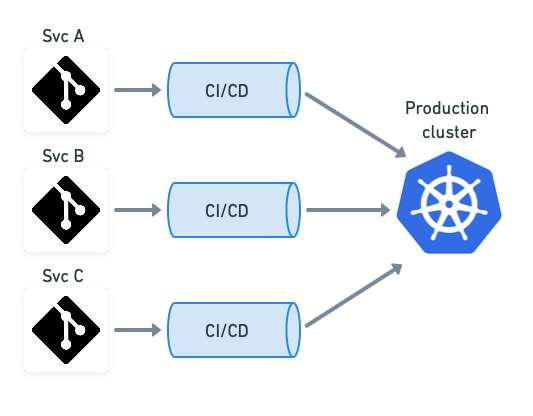
\includegraphics[width=\textwidth]{microdeployment.jpg}

For the moment, each repository will manage the GitFlow structure, and a
small modification will be made by adding a testing branch for the QA
team.

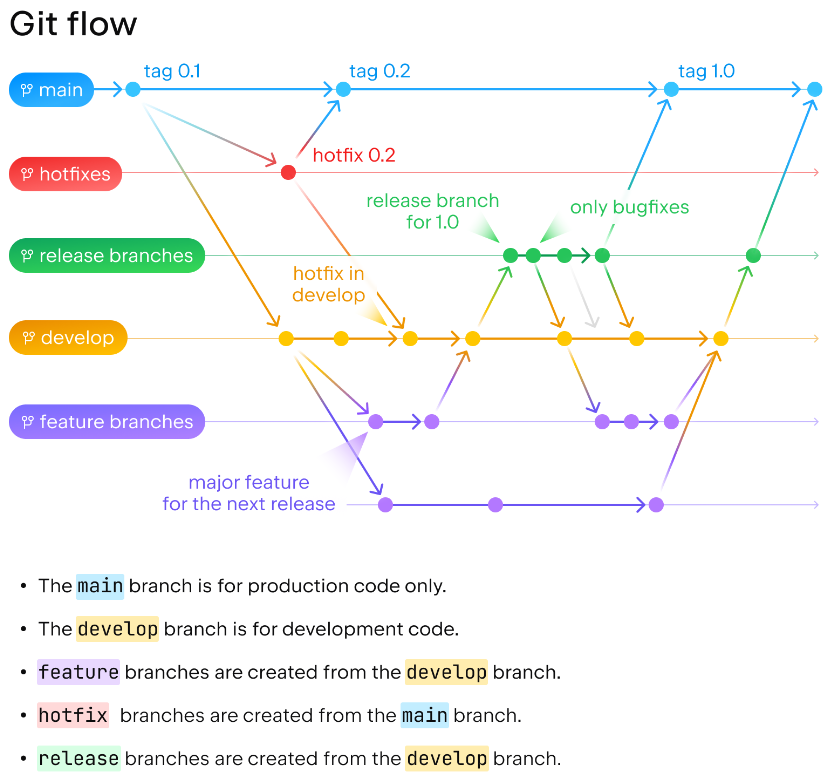
\includegraphics[width=\textwidth]{gitflow.png}

\hypertarget{conventionalcommits}{
\subsubsection{Conventional Commits:}\label{conventionalcommits}}

\emph{A specification for adding human and machine readable meaning to
commit messages}

\begin{enumerate}
\tightlist
\item
  \textbf{fix:} fixes a bug or defect.
\item
  \textbf{feat:} adds a new feature or functionality.
\item
  \textbf{build}: changes related to the build system or dependencies.
\item
  \textbf{chore:} maintenance or housekeeping tasks.
\item
  \textbf{ci:} changes to continuous integration.
\item
  \textbf{docs:} documentation changes.
\item
  \textbf{style:} code appearance or formatting changes.
\item
  \textbf{refactor:} significant code restructuring without behavior
  change.
\item
  \textbf{perf:} performance improvements.
\item
  \textbf{test:} changes related to testing.
\end{enumerate}

\hypertarget{pullrequeststructurenbsp}{
\subsubsection{Pull Request
structure:~}\label{pullrequeststructurenbsp}}

\begin{itemize}
\tightlist
\item
  \textbf{Pull Request Title:} Title should be clear and concise, and
  should accurately reflect the purpose of the change.
\item
  \textbf{Pull Request Description:} The description should provide
  details about what changes were made and why. You should include any
  relevant context that helps understand the change.

  \begin{itemize}
  \tightlist
  \item
    We will use the \textbf{Pull Request Template} and answer the
    following 3 questions:

    \begin{itemize}
    \tightlist
    \item
      What did I do?
    \item
      How did I do it?
    \item
      Why did I do it?
    \end{itemize}
  \end{itemize}
\item
  \textbf{References to Issues:} If the change is related to an issue in
  your issue tracking system (such as Jira, GitHub Issues, etc.), it
  should be mentioned in the description. This will help connect your
  pull request to the problem it is solving.
\item
  \textbf{Request Reviewers:} Ask one or more members of your team to
  review the pull request. They will provide feedback and suggest
  improvements if necessary.
\end{itemize}

\end{document}